\documentclass[twocolumn,letterpaper,12pt,notitlepage]{article}
\usepackage{graphicx}
\usepackage[font=bf]{caption}
\graphicspath{ {./images/} }

\begin{document}

\title{Lord Stanley Seekers}

\author{
  Crooks, Kevin\\
  \texttt{crooksk@colorado.edu}
  \and
  Lim, Brian\\
  \texttt{brian.lim@colorado.edu}
  \and
  May, Arthur\\
  \texttt{arthur.may@colorado.edu}
}


\twocolumn[
\begin{@twocolumnfalse}
\maketitle
\end{@twocolumnfalse}
]

\section{Problem Space}
In the world of sports, predicting a game’s outcome has myriad benefits. It can help coaches and players
learn what areas to focus on. It can help sportswriters write articles outlining the predictions for season-
final standings. It can help oddsmakers set profitable betting lines. Unfortunately for these professionals, current best NHL game prediction accuracy is less than 70 percent. This is generally attributed to simple
randomness in sports, the general perception of higher parity in the NHL as opposed to other sports (we
all know the Patriots are going to be in the postseason, right?), and of course the randomness of ice
condition. Bad bounces, breaks, millimetres in difference in skate angle, etc. Nonetheless, 70 percent isn’t bad,
but naturally everyone wants these to be better.  \newline

Rather than retreaded an old problem space, which would simply amount to wondering if the science has improved in the past few years, or training algorithms have, we decided to look at a new
problem: period prediction. An NHL game is divided into 3 periods of twenty minutes each. If the score
is still tied after these three regulation periods, a 4th  overtime period is played. Overtime rules have
changed a few times in the past couple of decades, but the current standard is a single 5-minute period.
We included these in our analyses as well. Despite the fact that statistics will be different between a full
20-minute period and a shorter 5-minute period, we are looking at predictors for each period individually,
so our overall models will not be affected by this bundling. \newline

The advantage to such a prediction might be immediately obvious to a coach, although probably
not as useful for Vegas. If your team enters the second period trailing by 2, how do you overcome that
lead? If hits have a high correlation with success, maybe play more aggressively. If blocked shots have a
low correlation, don’t worry about taking too many bad shots at the risk of turning the puck over. Our
goal is to see if we can find which statistics, taken from the standard metrics used in NHL statkeeping,
can be beneficial in predicting the outcome of a period.


Our approach to address the problem iterated through three steps over multiple phases. The first step was to prepare the data. Once the data was prepared, we performed a number of visualizations around the data to get an understanding of relationships between features and the end of period goal differential. Once we had an understanding of the relationships between the features, we ran them through different machine learning classifiers based on the results we were seeking. We did not seek a binary prediction, but a goal differential which is a bit more challenging.

Several classifiers will be tested including a gradient boost, random forest, and KNN. The classifier that performed the best will be used to present the results. 

\section{Data}

The data for this work was obtained from Kaggle, comprised of 3.6 million plays over 11,400 games over
the course of 3 full seasons. The plays including the standard stats recorded by the NHL – goals,
penalties, shots on goal, blocked shot, hits, faceoffs, takeaways, giveaways, and missed shots. This data
was synchronized with 8.9 million shifts for the same games (a shift is defined as a consecutive time on
ice for a player, typically 20-40 seconds, and a player might have 40 shifts over the course of a single
game). This data was then split by home and away, the artificial split we used as the easiest way to
differentiate teams. Concordantly, the predicted outcome, final period goal differential, was also given as
Away minus Home. Thus to determine final goal differential for the away team, simply take the negative
of the result. The resultant feature matrix was 37589x19: 37,589 periods for which we had valid
statistics and 19 statistical measurements, originally given as raw counts to be later normalized and
scaled depending on the statistic in question. A sample of the data can be found in Table \ref{tab:1}. \newline

A small handful of periods had to be rejected from having missing statistics, or obviously incorrect
statistics. This generally happened in overtime periods for some unknown reason. Additionally, we noted
a minor statistical error, probably attributed to typographical errors at the input level, in which a player’s
shift length was given as 1-2 seconds, followed by a regular 30 second shift. The number of these was
small enough that they were included regardless, reasoning they would have little effect on the overall
average shift length feature, and indeed in the final outcome itself.

\begin{table*}[t]
  \centering
  \resizebox{\textwidth}{!}{\begin{tabular}{||c c c c c c c c||}
    \hline
periodID & period initial goal differential & blocked shots away & blocked shots home & faceoff away & faceoff home & ... &  period final goal differential \\ [0.5ex] 
 	\hline\hline	
    2010020001\_1 & 0 & 7 & 6 & 9 & 5 & ... & 1 \\
    \hline
    2010020001\_2 & 1 & 8 & 13 & 5 & 8 & ... & 0 \\
    \hline
    2010020001\_3 & 1 & 6 & 3 & 9 & 7 & ... & 0 \\ [1ex]
    \hline
  \end{tabular}}
  \caption{NHL game data prepared sample}
  \label{tab:1}
\end{table*}

After preparing the data, a number of visualizations were performed to better understand the relationships. 

Figure \ref{fig:1} contains a Seabornviolin plot. In this particular plot the difference between the home and away value of each attribute against the change in goal differential at the beginning and ending of the period. The penalty differential and takeaway differential appeared to have a strong relationship which makes sense. If you are on a powerplay more than your opponent in a period, you will have more goals. Same argument can be made for takeaways. Nonetheless, some attributes had more impact on the outcome than others.

The same analysis was done attribute by attribute using a Seaborn joint plot. A sample plot can be found in Figure \ref{fig:2}.

\begin{figure}[htp]
\centering
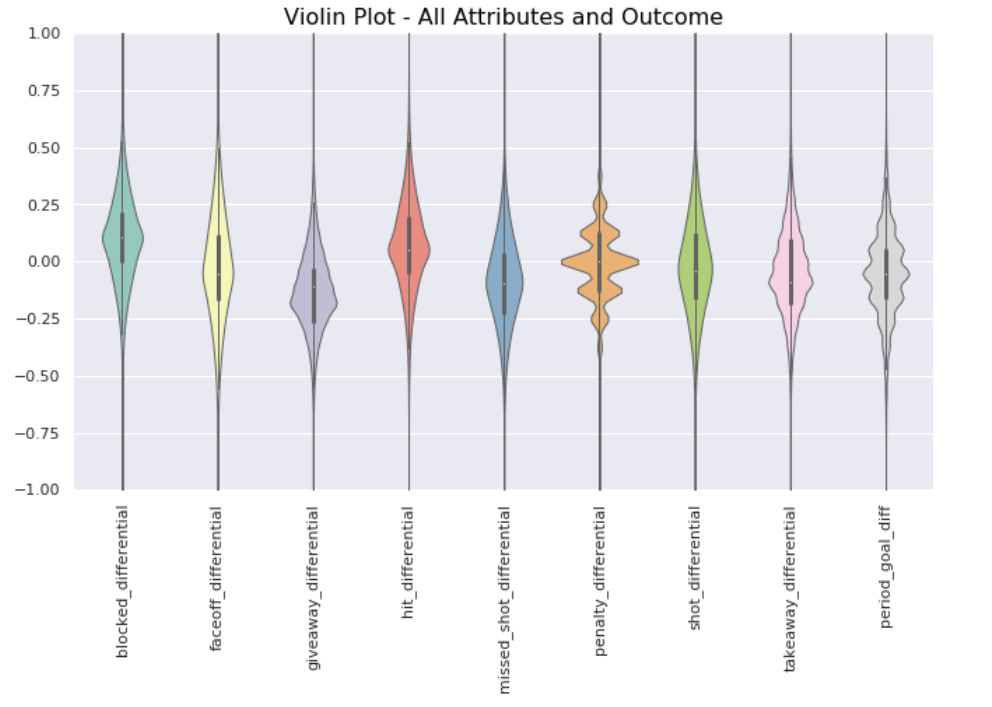
\includegraphics[width=\linewidth]{violin}
\caption{Violin plot of difference between home and away attributes vs. Outcome}
\label{fig:1}
\end{figure}

\begin{figure}[htp]
\centering
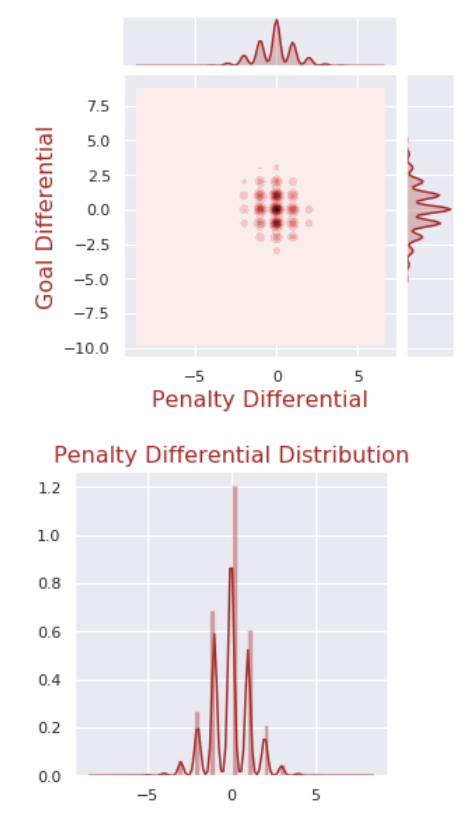
\includegraphics[width=\linewidth]{joint}
\caption{Joint plot of penalty differential and goal differential for the period}
\label{fig:2}
\end{figure}


\section{Results}
Clearly present the results of your efforts. Include all measures you deem appropriate (e.g. accuracy, sources of error, ROC curves, feature weights, etc.). Include comparisons to baseline data and results from prior work where appropriate.

\section{Discussion}
Present your interpretation of the results. Discuss how these results might have an impact on the field - or discuss how they might suggest other directions to investigate. Discuss potential future plans for this work (even if you don't actually plan to follow up on them).


\end{document}







